\chapter{A LUZ COMO MATERIAL E O CUBO PRETO}

Segundo \citeonline[p. 1]{azevedo} a problemática da luz atravessa a história da arte, de finais do século XIX e durante o século XX. A função da luz não é mais somente de iluminar, de tornar visível uma obra ou um objeto, ou o mero reflexo dos seus efeitos suspensos no espaço. A luz passa a ser tratada como objeto ou material. Na perspectiva da arte contemporânea, se vê que, em muitas obras, a luz passa à matéria. \citeonline[p. 50]{brandi} destaca que "alguns artistas e movimentos estéticos estão fortemente relacionados com a linguagem da luz, mesmo quando não a utilizam como objeto central da obra". 

De acordo com \citeonline[p. 18]{vega} os artistas, em diferentes épocas, se viram inspirados e cativados pela luz, tanto a natural quanto a artificial, e tentaram capturar seu mistério e sua natureza mágica em suas criações. Alguns em particular, como Caravaggio, Vermeer e Monet, buscaram retratar, quase como uma obsessão, a luz e seus efeitos no mundo ao seu redor e, mais recentemente, os artistas contemporâneos vem se utilizando da luz como matéria-prima, realizando manipulações em três dimensões para projetar suas dimensões infinitas. \citeonline[p. 23]{vega} afirma também que, atualmente, muitos artistas exploram as possibilidades da luz artificial, trabalhando com mescla de materiais e diversos tipos de fontes de luz. 

James Turrell, por exemplo, foi pioneiro de uma nova preocupação com os fenômenos do espaço e da luz. Em seus primeiros trabalhos investigou os efeitos da luz artificial. Ele também desenvolveu várias instalações que aumentaram a relação entre a luz e a estrutura arquitetônica. Em conversa com \citeonline[p. 114]{adcock}, ele relata que uma das dificuldades de usar a luz é que ainda não é tradição utilizá-la em nossa cultura. Por outro lado, não é mais incomum usá-la do que usar pedra, argila, aço ou tinta. O artista declara seu interessa em trabalhar a luz como material, mas não luz em vidro, fibra de vidro ou acrílico, e sim no próprio espaço e nas qualidades do espaço, fazendo luz sem a forma física tradicional. Ele nos traz também que há uma rica tradição na pintura do trabalho sobre a luz, mas que isso de fato não é luz - é o registro da visão. Na figura \ref{fig:james_turrell} podemos ver sua obra entitulada \textit{The light inside} que transforma as paredes de um túnel em vasos para a condução da luz e nos dá uma ideia da dimensão em que o artista trabalha este material. 

\begin{figure}[H]
    \centering
    \caption{The light inside, James Turrell, 1999}
	\vspace*{0,2cm}
    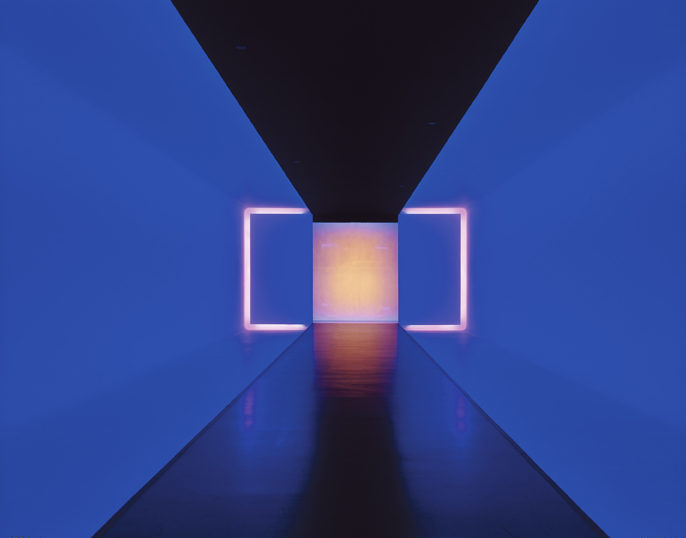
\includegraphics[width=0.8\textwidth]{./04-figuras/james_turrell}
    \label{fig:james_turrell}
\end{figure}
\vspace*{-0,9cm}
{\raggedright \fonte{Disponível em: <http://jamesturrell.com/work/thelightinside/>. Acesso em: 18 jun. 2018}}\\


Outro artista cuja obra é relevante no contexto deste trabalho é o japonês Takahito Matsuo que, segundo \citeonline[p. 5]{soares}, cria mundos interativos de fantasia e de luz que fazem parte de uma estética enigmática, misturando som e luz perante os movimentos do observador. Seu trabalho destaca as diferentes gradações de luz e sombra que contrastando mostram um mundo de fantasia e imaginação. Em \textit{Fantasias Aquáticas Iluminadas} (figura \ref{fig:takahito_matsuo}), a exploração através de luz, projeções, arquitetura e interações humanas é fortemente encorajada. À medida que os visitantes se aproximam das paredes, se movimentam e se afastam, o número e a frequência das medusas aumentam e diminuem. As formas orgânicas e a brilhante paleta de azúis criam um mundo subaquático surreal, onde movimentos lúdicos e interações com o espaço arquitetônico resultam em uma comunicação não dita entre artista e participante. 

\begin{figure}[H]
    \centering
    \caption{Fantasias Aquáticas Iluminadas, Takahito Matsuo, 2009}
	\vspace*{0,2cm}
    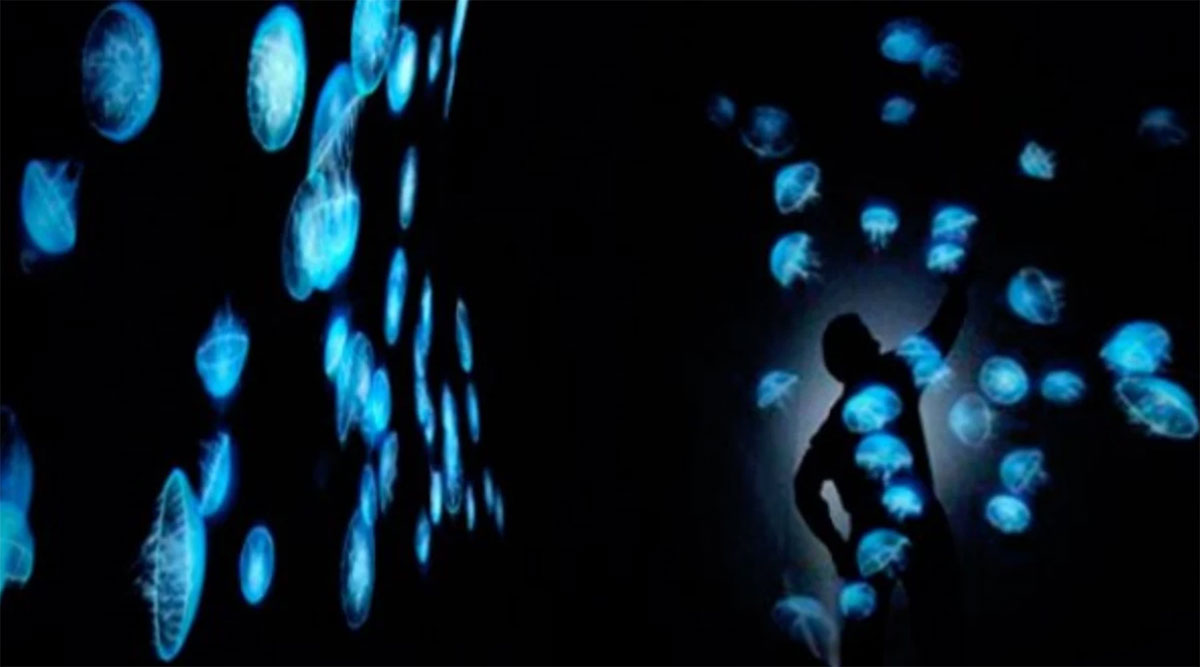
\includegraphics[width=0.8\textwidth]{./04-figuras/takahito_matsuo}
    \label{fig:takahito_matsuo}
\end{figure}
\vspace*{-0,9cm}
{\raggedright \fonte{\citeonline{soares}}}\\

A figura \ref{fig:jim_campbell} mostra o trabalho do artista Jim Campbell que, em um mundo de alta definição e telas cada vez mais finas, usa tecnologia para produzir o contrário: imagens borradas e em baixa resolução em painéis tridimensionais. Essas video-esculturas são compostas por grades de LEDs que atuam como uma televisão de pixels desconstruída. 

\begin{figure}[H]
    \centering
    \caption{Light Topography Wave, Jim Campbell, 2014}
	\vspace*{0,2cm}
    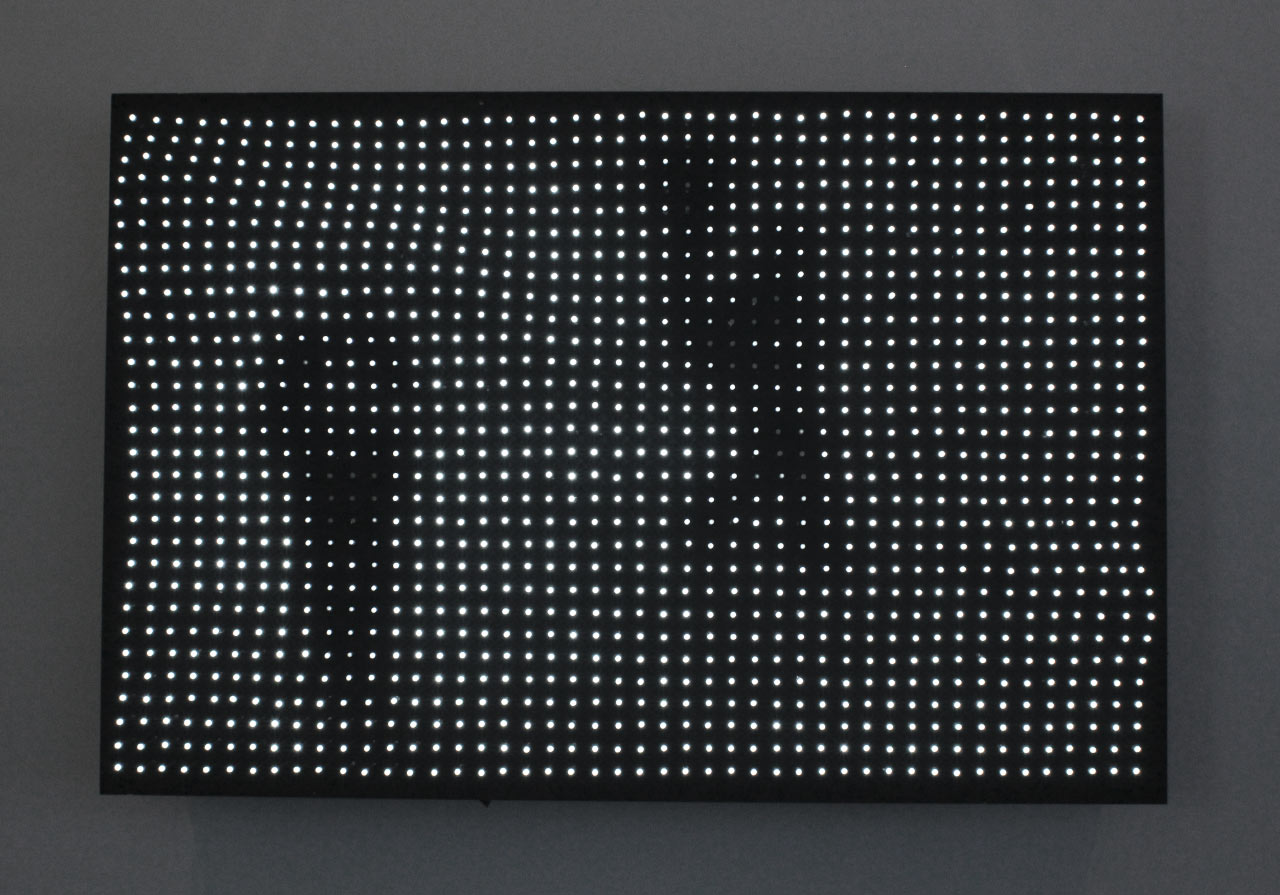
\includegraphics[width=0.8\textwidth]{./04-figuras/jim_campbell}
    \label{fig:jim_campbell}
\end{figure}
\vspace*{-0,9cm}
{\raggedright \fonte{Disponível em: <https://design-milk.com/pixelated-led-art-jim-campbell/>. Acesso em: 22 mar. 2018}}\\

Do ponto de vista da propagação da luz, o cubo branco tende a não ser o cenário ideal para exibição da obra. Além disso, \citeonline[p. 40]{soares}, afirma que "a maioria dos autores que trabalham com arte e tecnologia procuram o espaço do cubo preto como espaço expositivo. Neste espaço o que interessa é um novo ver, um espanto com a imagem". Diz ainda que o nome cubo preto para este tipo de exposição surge em contraposição ao cubo branco, criado por Brian O'Doherty, num ensaio publicado pela revista Artforum em 1976, fazendo alusão ao espaço das galerias de arte, com paredes brancas, sem janelas isolando o espetador num meio aparentemente atemporal. A ideia do cubo preto surge como ambiente ideal para propagação da luz e é também uma forma de imersão no interior da mente do artista.
